% ARI v0.2 rewrite — SKELETON DRAFT (bullets, tables, figures; prose comes later).
% Scope: ARI-R (embeddings) and ARI-D (generation). Target: 6 pages + appendix.
% Numbers: v0.2 reruns where finished. Values marked with \pend{} are v0.1 placeholders
% awaiting the v0.2 rerun (API panel: 2026-10-09; H100: 2026-10-13).
\documentclass{article}
\usepackage[final,sglblindworkshop]{neurips_2026}
\workshoptitle{Machine Learning for Systems}
\usepackage[utf8]{inputenc}
\usepackage[T1]{fontenc}
\usepackage[hypertexnames=false]{hyperref}
\usepackage{url,booktabs,graphicx,amsmath,amssymb,xcolor,enumitem}
\usepackage{pgfplots}
\usepackage{tikz}
\usetikzlibrary{positioning,arrows.meta,shapes.misc}
\pgfplotsset{compat=1.18}
\hypersetup{hidelinks}
\setlist{nosep,leftmargin=1.2em}
\definecolor{sOne}{HTML}{2A78D6}   % code / v0.2 probe
\definecolor{sTwo}{HTML}{EB6834}   % hash / raw bytes / calibrated
\definecolor{sThree}{HTML}{1BAF7A}
\definecolor{inkMuted}{HTML}{7A808A}
\newcommand{\pend}[1]{\textcolor{inkMuted}{#1}\textsuperscript{\textcolor{inkMuted}{\dag}}}
\newcommand{\todo}[1]{\textcolor{sTwo}{\textbf{[#1]}}}
\newcommand{\rhoc}{\rho}

\title{ARI: Measuring Whether a Hosted Model Returns the Same Output Twice}
\author{The SEMQ Group}

\begin{document}
\maketitle

\begin{abstract}
Sending the same input to the same hosted model does not guarantee the same output, and providers do not report how often outputs change. We present the AI Reproducibility Index (ARI), a black-box protocol that measures output reproducibility under conditions any user can induce: a fresh process, concurrent load, and a gap of more than 24 hours. ARI-R measures embedding models by encoding each vector with a public, calibration-free quantizer and reporting two numbers per condition: the exact-match rate and a dimension-normalized coordinate change rate. ARI-D measures generation endpoints by byte-identical repeats. Against ground-truth vectors from eight encoders, the quantizer ignores floating-point jitter that changes the bytes of 2--100\% of vectors, changes the codes of 99--100\% of vectors under precision changes, and its change rate does not depend on dimension between 384 and 1{,}024. Across five embedding APIs, exact-match agreement ranges from \pend{0.169} to \pend{1.000}; across five generation endpoints, byte-identical repeat rates range from 0.107 to 1.000, and a gateway serving the vendor's model snapshot is less stable than the vendor API. Self-hosted fp32 inference is bit-reproducible across processes and threads and agrees at $\ge$0.996 across GPU models, while enabling TF32 changes 54\% of document codes with no detectable change in Recall@10. ARI gives practitioners a fixed procedure, signed reports, and two numbers that answer how reproducible their model is.
\end{abstract}

%=====================================================================
\section{Introduction}\label{sec:intro}
\textbf{Problem.}
\begin{itemize}
  \item Same input + same hosted model $\not\Rightarrow$ same output: batching, kernel choice, precision tiers and backend changes alter numerics [1, 2, 8].
  \item Providers publish no reproducibility numbers; users cannot see backend state.
  \item Task metrics (Recall@10, accuracy) do not register numerical change (\S\ref{sec:retrieval}).
\end{itemize}
\textbf{Who needs a number.}
\begin{itemize}
  \item Systems that \emph{store} a function of the output: cache keys, dedup hashes, semantic IDs [3], vector indexes built once and queried later.
  \item Audits and regulated pipelines that must re-derive a past result.
  \item Teams choosing a provider, a precision tier or a serving stack.
\end{itemize}
\textbf{Contributions.}
\begin{enumerate}[label=(\arabic*)]
  \item \textbf{ARI-R}: a protocol and two metrics for embedding reproducibility --- exact-match rate (HER) and a dimension-normalized change rate ($\rhoc$) --- on a public, calibration-free quantizer validated against ground truth (\S\ref{sec:arir}).
  \item \textbf{ARI-D}: the same conditions applied to generation endpoints, scored on byte-identical repeats, with no probe (\S\ref{sec:arid}).
  \item \textbf{Measurements}: five embedding APIs, eight self-hosted encoders on CPU and three GPU architectures, five generation endpoints; plus a practitioner guide (\S\ref{sec:use}).
\end{enumerate}

%=====================================================================
\section{The ARI protocol}\label{sec:protocol}
\begin{figure}[h]
\centering
\resizebox{\linewidth}{!}{%
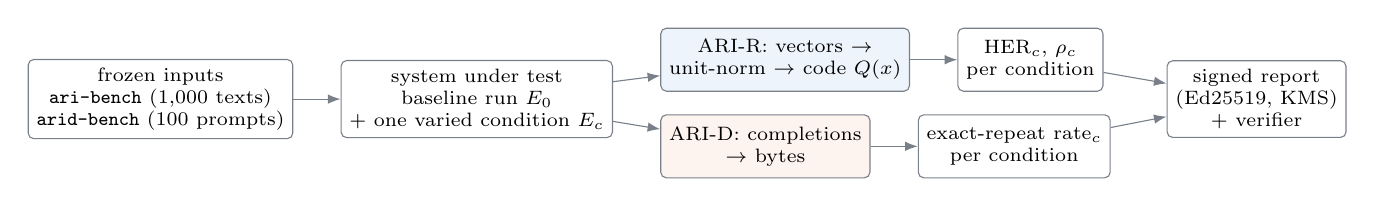
\begin{tikzpicture}[node distance=4mm and 6mm, every node/.style={font=\scriptsize},
  box/.style={draw=inkMuted, rounded corners=2pt, inner sep=3pt, align=center, minimum height=8mm},
  arr/.style={-{Latex[length=1.6mm]}, draw=inkMuted}]
\node[box] (in) {frozen inputs\\ \texttt{ari-bench} (1{,}000 texts)\\ \texttt{arid-bench} (100 prompts)};
\node[box, right=of in] (sys) {system under test\\ baseline run $E_0$\\ + one varied condition $E_c$};
\node[box, right=of sys, yshift=5mm, fill=sOne!8] (r) {ARI-R: vectors $\to$\\ unit-norm $\to$ code $Q(x)$};
\node[box, right=of sys, yshift=-6mm, fill=sTwo!8] (d) {ARI-D: completions\\ $\to$ bytes};
\node[box, right=of r] (rm) {HER$_c$, $\rho_c$\\ per condition};
\node[box, right=of d] (dm) {exact-repeat rate$_c$\\ per condition};
\node[box, right=8mm of rm, yshift=-5mm] (rep) {signed report\\ (Ed25519, KMS)\\ + verifier};
\draw[arr] (in) -- (sys); \draw[arr] (sys) -- (r); \draw[arr] (sys) -- (d);
\draw[arr] (r) -- (rm); \draw[arr] (d) -- (dm); \draw[arr] (rm) -- (rep); \draw[arr] (dm) -- (rep);
\end{tikzpicture}}
\caption{ARI pipeline. One baseline, one varied condition at a time, frozen hash-pinned inputs, a signed report anyone can verify without our code.}\label{fig:pipeline}
\end{figure}

\begin{table}[h]\centering\footnotesize
\caption{Conditions. The core (bold) is externally inducible on any hosted API.}\label{tab:conditions}
\begin{tabular}{llll}
\toprule
condition & what changes & question it answers & who can run it \\
\midrule
\texttt{same} & nothing (immediate repeat) & control & everyone \\
\textbf{\texttt{proc}} & fresh process / client & ``is a restart safe?'' & everyone \\
\textbf{\texttt{conc}} & 64-way burst vs calm & ``does load change my output?'' & everyone \\
\textbf{\texttt{time}} & gap $>24$\,h (we use $\sim$76\,h) & ``will it match next week?'' & everyone \\
\texttt{mach} & host / GPU & portability & self-hosted \\
\texttt{prec} & bf16, fp16, int8, TF32 & serving-tier effect & self-hosted \\
\bottomrule
\end{tabular}
\end{table}
\begin{itemize}
  \item One execution pair per condition; bootstrap CIs over inputs (not over serving realizations).
  \item Report carries: per-condition metrics, environment manifest, input content hash, audit digest of codes, signature.
  \item \todo{burst size and Mistral exception written into spec/condition-set.md}
\end{itemize}

%=====================================================================
\section{ARI-R: embedding reproducibility}\label{sec:arir}
\subsection{The probe}
\begin{itemize}
  \item Rescale each vector to unit norm; encode with SEMQ QUANT (public SDK, \texttt{semq==1.0.0}): per coordinate, sign + magnitude bin over the fixed range $2/\sqrt d$; 2 bits/coordinate.
  \item No calibration: the range depends on $d$ only, so any party computes identical codes from identical vectors (byte-identical across CPUs and language bindings).
  \item Why fixed, not calibrated: re-calibrating the old probe on a different corpus slice moved the scale by 0.3--3.6\% and \textbf{changed 60--100\% of codes for identical vectors} (App.~\ref{app:probe}).
\end{itemize}
\textbf{Why a quantizer and not a hash.}
\begin{itemize}
  \item \textbf{Ignores sub-threshold noise.} A hash flags any bit change; the code flags a change only when a coordinate crosses a bin edge (Fig.~\ref{fig:selectivity}).
  \item \textbf{Locates what moved.} Codes are per-coordinate, so a diff names the coordinates and inputs that changed; a hash says only ``different''.
  \item \textbf{Discrete stored state.} 2 bits/dim (16$\times$ smaller than fp32); a baseline can be stored, content-addressed and signed, then compared later without keeping vectors.
\end{itemize}
\begin{table}[h]\centering\footnotesize
\caption{What each stored artifact can answer, per 1{,}024-d vector.}\label{tab:storage}
\begin{tabular}{lrccc}
\toprule
artifact & bytes & detects change & ignores jitter & locates change \\
\midrule
SHA-256 of fp32 bytes & 32 & yes, any bit & no & no \\
ARI-R code ($n_{\text{bins}}{=}2$) & 256 & above bin edge & yes & yes (coordinate) \\
fp32 vector & 4{,}096 & yes, exact & no & yes (exact value) \\
\bottomrule
\end{tabular}
\end{table}

\subsection{Metrics: HER and $\rho$}\label{sec:metrics}
\begin{itemize}
  \item $\mathrm{HER}_c$ = fraction of inputs whose \emph{whole} code matches. Answers ``will my stored key/ID still match?''
  \item $\rho_c$ = fraction of \emph{coordinates} whose symbol changed, averaged over inputs. Answers ``how much does the output move?''
  \item \textbf{HER depends on dimension, $\rho$ does not} (Fig.~\ref{fig:dim}): at equal noise, HER falls from 0.64 (384-d) to 0.26--0.32 (1{,}024-d) while $\rho$ stays at $1.1$--$1.4\times10^{-3}$.
  \item \textbf{Headline score} $\text{ARI-R} = 1 - \overline{\rho}_{\{\texttt{proc},\texttt{conc},\texttt{time}\}}$ (dimension-normalized; use to compare models). HER is reported per condition alongside.
  \item Limits of normalization: holds for 384--1{,}024-d under isotropic relative noise; \todo{verify at 1{,}536 and 3{,}072-d on API data}; models with many near-zero coordinates flip signs more easily.
\end{itemize}

\begin{figure}[h]\centering
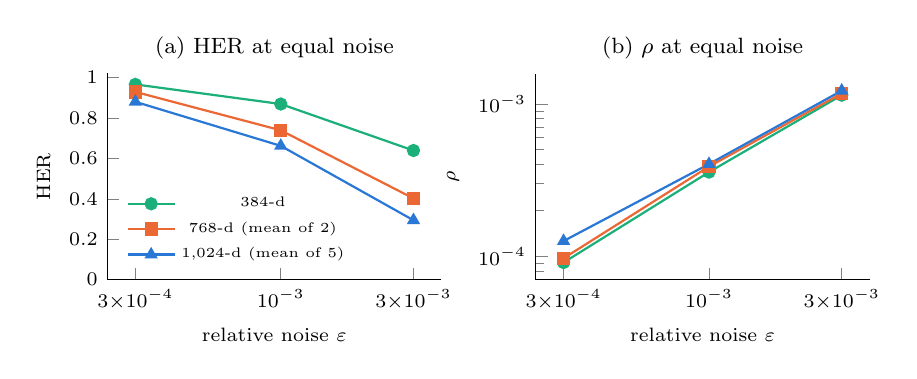
\begin{tikzpicture}
\begin{axis}[name=a, width=0.48\linewidth, height=4.2cm, xmode=log, xlabel={relative noise $\varepsilon$}, ylabel={HER}, ymin=0, ymax=1.02,
  title={\footnotesize (a) HER at equal noise}, title style={yshift=-1ex}, tick label style={font=\scriptsize}, label style={font=\scriptsize},
  legend style={font=\tiny, at={(0.03,0.03)}, anchor=south west, draw=none, fill=none}, xtick={3e-4,1e-3,3e-3}, xticklabels={$3{\times}10^{-4}$,$10^{-3}$,$3{\times}10^{-3}$}, axis x line*=bottom, axis y line*=left]
\addplot[sThree, thick, mark=*] coordinates {(3e-4,0.966)(1e-3,0.869)(3e-3,0.639)}; \addlegendentry{384-d}
\addplot[sTwo, thick, mark=square*] coordinates {(3e-4,0.929)(1e-3,0.739)(3e-3,0.402)}; \addlegendentry{768-d (mean of 2)}
\addplot[sOne, thick, mark=triangle*] coordinates {(3e-4,0.880)(1e-3,0.662)(3e-3,0.294)}; \addlegendentry{1{,}024-d (mean of 5)}
\end{axis}
\begin{axis}[at={(a.east)}, anchor=west, xshift=1.2cm, width=0.48\linewidth, height=4.2cm, xmode=log, ymode=log, xlabel={relative noise $\varepsilon$}, ylabel={$\rho$},
  title={\footnotesize (b) $\rho$ at equal noise}, title style={yshift=-1ex}, tick label style={font=\scriptsize}, label style={font=\scriptsize}, xtick={3e-4,1e-3,3e-3}, xticklabels={$3{\times}10^{-4}$,$10^{-3}$,$3{\times}10^{-3}$}, axis x line*=bottom, axis y line*=left]
\addplot[sThree, thick, mark=*] coordinates {(3e-4,9.11e-5)(1e-3,3.57e-4)(3e-3,1.14e-3)};
\addplot[sTwo, thick, mark=square*] coordinates {(3e-4,9.71e-5)(1e-3,3.88e-4)(3e-3,1.17e-3)};
\addplot[sOne, thick, mark=triangle*] coordinates {(3e-4,1.26e-4)(1e-3,4.03e-4)(3e-3,1.22e-3)};
\end{axis}
\end{tikzpicture}
\caption{Same noise, eight encoders. HER falls with dimension; $\rho$ does not. Synthetic per-coordinate relative noise on 1{,}000 frozen inputs, v0.2 probe.}\label{fig:dim}
\end{figure}

\subsection{Validation against ground truth}
\begin{itemize}
  \item Raw float32 vectors from 8 encoders, 1{,}000 inputs, reference fp32/CPU/4 threads/batch 32, one varied condition per fresh process; ``changed'' = any byte differs.
  \item 0 false positives: no unchanged vector ever changed code.
  \item Code change tracks true L2 drift (Spearman 0.88--0.95 per model).
\end{itemize}
\begin{figure}[h]\centering
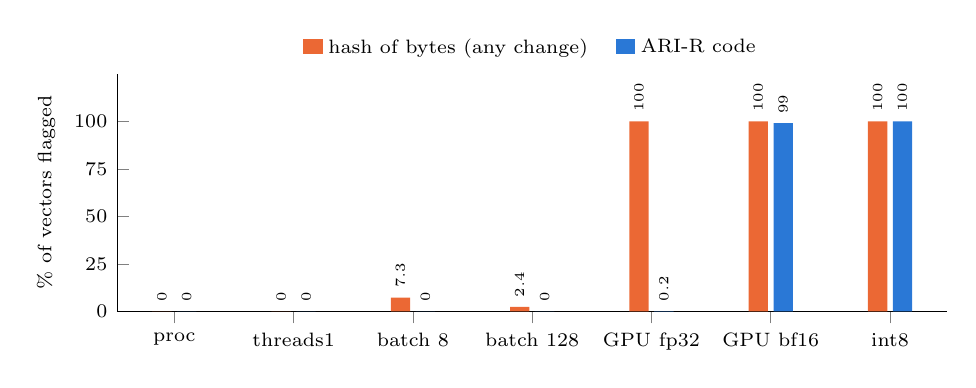
\begin{tikzpicture}
\begin{axis}[ybar, bar width=7pt, width=\linewidth, height=4.6cm, ymin=0, ylabel={\% of vectors flagged},
  symbolic x coords={proc,threads1,batch 8,batch 128,GPU fp32,GPU bf16,int8}, xtick=data,
  tick label style={font=\scriptsize}, label style={font=\scriptsize}, enlarge x limits=0.08, axis x line*=bottom, axis y line*=left,
  legend style={font=\scriptsize, at={(0.5,1.02)}, anchor=south, draw=none, fill=none, /tikz/every even column/.append style={column sep=8pt}}, legend columns=2,
  legend image code/.code={\draw[#1, draw=none] (0cm,-0.08cm) rectangle (0.25cm,0.12cm);},
  nodes near coords, nodes near coords style={font=\tiny, rotate=90, anchor=west, /pgf/number format/fixed, /pgf/number format/precision=1}, ymax=125, ytick={0,25,50,75,100}]
\addplot[fill=sTwo, draw=none] coordinates {(proc,0)(threads1,0)(batch 8,7.3)(batch 128,2.36)(GPU fp32,100)(GPU bf16,100)(int8,100)};
\addplot[fill=sOne, draw=none] coordinates {(proc,0)(threads1,0)(batch 8,0)(batch 128,0)(GPU fp32,0.18)(GPU bf16,99.0)(int8,100)};
\legend{hash of bytes (any change), ARI-R code}
\end{axis}
\end{tikzpicture}
\caption{Selectivity, mean over 8 encoders. Batch-size and CPU$\to$GPU fp32 jitter change bytes but not codes; precision changes are flagged. GPU = Apple M5 Max.}\label{fig:selectivity}
\end{figure}

%=====================================================================
\section{ARI-R findings}\label{sec:arir-findings}
\subsection{Hosted embedding APIs}
\begin{table}[h]\centering\footnotesize
\caption{Five embedding APIs, 1{,}000 frozen inputs. \pend{} = v0.1 placeholder, v0.2 rerun 2026-10-09 (adds $\rho$).}\label{tab:api}
\begin{tabular}{lrrrrrr}
\toprule
model & $d$ & HER \texttt{proc} & HER \texttt{conc} & HER \texttt{time} & ARI-R ($1-\bar\rho$) & 95\% CI \\
\midrule
gemini-embedding-001 & 3072 & \pend{1.000} & \pend{1.000} & \pend{1.000} & \todo{} & \todo{} \\
text-embedding-3-large & 3072 & \pend{0.862} & \pend{0.851} & \pend{0.822} & \todo{} & \todo{} \\
mistral-embed & 1024 & \pend{0.753} & \pend{0.791} & \pend{0.554} & \todo{} & \todo{} \\
voyage-4-large & 1024 & \pend{0.615} & \pend{0.209} & \pend{0.676} & \todo{} & \todo{} \\
embed-v4.0 & 1536 & \pend{0.146} & \pend{0.130} & \pend{0.232} & \todo{} & \todo{} \\
\bottomrule
\end{tabular}
\end{table}
\begin{itemize}
  \item Conditions expose different failures: one provider collapses only under concurrency (\pend{0.209}), another only after the multi-day gap (\pend{0.554}); one is bit-identical in every condition.
  \item Drifting providers move many coordinates at small magnitude ($\sim$2{,}300 of 3{,}072 dims at $\sim10^{-4}$) $\Rightarrow$ backend numerics, not last-bit noise.
  \item Rank providers only on ARI-R ($\rho$), never on HER. \todo{figure: dot plot, one row per model, marks for proc/conc/time}
\end{itemize}

\subsection{Self-hosted encoders}
\begin{table}[h]\centering\footnotesize
\caption{Eight encoders (384--1{,}024-d), v0.2 rerun. HER per condition; GPU rows n = 512.}\label{tab:selfhosted}
\begin{tabular}{llr}
\toprule
condition & setting & HER (range over 8 encoders) \\
\midrule
\texttt{proc}, threads, batch & CPU fp32 & 1.000 \\
\texttt{proc} & A10G / T4 fp32, TF32 off & 1.000 \\
\texttt{mach} & A10G $\leftrightarrow$ T4, fp32 & 0.996--1.000 \\
\texttt{proc} & A10G fp32, \textbf{TF32 on} & \textbf{0.594--0.848} (mean 0.725) \\
\texttt{prec} & bf16 / int8 (CPU) & \todo{CPU panel; locally 0.000--0.069} \\
\texttt{conc}, \texttt{time} (>24\,h) & CPU & \todo{2026-10-07} \\
\midrule
\texttt{proc} / \texttt{conc} / \texttt{prec} & SFR-Embedding-2\_R (7B, 4{,}096-d), L40S fp32$^\ast$ & 1.000 / \textbf{0.998} / 0.000 \\
batch 1 vs 32 & H100 & \todo{2026-10-13} \\
\bottomrule
\end{tabular}
\end{table}
\begin{figure}[h]\centering
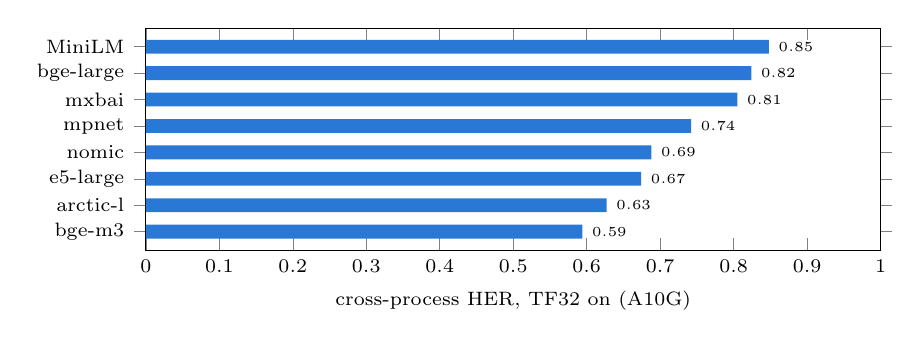
\begin{tikzpicture}
\begin{axis}[xbar, bar width=5pt, width=0.9\linewidth, height=4.4cm, xmin=0, xmax=1, xlabel={cross-process HER, TF32 on (A10G)},
  symbolic y coords={bge-m3,arctic-l,e5-large,nomic,mpnet,mxbai,bge-large,MiniLM}, ytick=data,
  tick label style={font=\scriptsize}, label style={font=\scriptsize}, nodes near coords, nodes near coords style={font=\tiny}]
\addplot[fill=sOne, draw=none] coordinates {(0.594,bge-m3)(0.627,arctic-l)(0.674,e5-large)(0.688,nomic)(0.742,mpnet)(0.805,mxbai)(0.824,bge-large)(0.848,MiniLM)};
\end{axis}
\end{tikzpicture}
\caption{TF32 alone breaks cross-process reproducibility; TF32 off gives 1.000 for all eight; \texttt{use\_deterministic\_algorithms} has no effect (identical values).}\label{fig:tf32}
\end{figure}
\begin{itemize}
  \item Pinning precision (fp32, TF32 off) $\Rightarrow$ bit-reproducible across process and threads; $\ge$0.996 across GPU models.
  \item Exposed axis is CPU$\leftrightarrow$GPU and TF32; portable axis is GPU$\leftrightarrow$GPU.
  \item Concurrent encoding on one shared model instance is not perfectly reproducible: SFR \texttt{conc} = 0.998 (2 of 1{,}000 inputs). $^\ast$fp32 compute on bf16-loaded weights.
\end{itemize}

\subsection{Task metrics do not register the change}\label{sec:retrieval}
\begin{table}[h]\centering\footnotesize
\caption{BEIR SciFact (5{,}183 docs, 300 judged queries), all-MiniLM-L6-v2, v0.2. \todo{rerun at $n_{\text{bins}}{=}2$ to match the ARI-R probe (currently 8 bins)}.}\label{tab:scifact}
\begin{tabular}{lrrrr}
\toprule
condition & codes changed & $\Delta$R@10 & 95\% CI & top-10 same \\
\midrule
proc / threads / batch 8 / 128 & 0\% & 0.000 & [0, 0] & 100\% \\
GPU fp32, TF32 off & 0.1\% & 0.000 & [0, 0] & 100\% \\
GPU fp32, \textbf{TF32 on} & \textbf{54\%} & 0.000 & [0, 0] & 96\% \\
GPU fp16 & 100\% & 0.000 & [0, 0] & 93\% \\
bf16, CPU & 100\% & +0.003 & [0, 0.010] & 45\% \\
bf16, GPU & 100\% & $-$0.003 & [$-$0.010, 0] & 43\% \\
int8 (CPU) & 100\% & $-$0.006 & [$-$0.028, 0.016] & 0\% \\
\bottomrule
\end{tabular}
\end{table}
\begin{itemize}
  \item Numerical change is real but tiny (dot products $\approx$ 1.0000); Recall@10 is invariant to it, codes are not.
  \item Claim is \emph{not} ``retrieval misses large drift''; it is ``task metrics cannot tell you whether outputs are reproducible''.
\end{itemize}

\subsection{Case study: a silent precision change}
\begin{itemize}
  \item mxbai-embed-large-v1 declares \texttt{float16} in its config; transformers 5 loads the declared dtype unless told otherwise.
  \item An ``fp32'' pipeline ran it in fp16: 12{,}130 distinct coordinate values in 1M (vs 1{,}009{,}495 in fp32); CPU vs GPU HER $\approx$0.5 (fp16) vs 0.999 (fp32).
  \item ARI surfaced it as an outlier; a library default, not the model or hardware, caused it. \todo{one-panel figure}
\end{itemize}

%=====================================================================
\section{ARI-D: generation reproducibility}\label{sec:arid}
\begin{itemize}
  \item 100 frozen prompts (5 buckets), temperature 0 (+ seed where accepted), $k=8$ repeats per condition ($k=12$ under burst).
  \item Score: fraction of repeat \emph{pairs} with byte-identical completions, averaged over prompts; bootstrap CI over prompts.
  \item No quantizer: bytes are what an API user observes; anyone can check it.
\end{itemize}
\begin{table}[h]\centering\footnotesize
\caption{Byte-identical repeat rate, 5 endpoints (dry run). Superscript = achieved burst.}\label{tab:arid}
\begin{tabular}{llrrrrr}
\toprule
endpoint & class & \texttt{same} & \texttt{proc} & \texttt{conc} & \texttt{time} & ARI-D \\
\midrule
gemini-3.6-flash & vendor & 1.000 & 1.000 & 1.000$^{64}$ & \todo{} & \todo{} \\
mistral-medium-2604 & vendor & 0.525 & 0.550 & 0.432$^{16}$ & \todo{} & \todo{} \\
gpt-4o-mini & vendor & 0.470 & 0.443 & 0.479$^{64}$ & 0.469 & 0.464 \\
Llama-3.3-70B-Turbo & rehosted & 0.452 & 0.431 & 0.448$^{64}$ & 0.435 & 0.438 \\
gpt-4o-mini & platform & 0.107 & 0.115 & --- & 0.109 & --- \\
\bottomrule
\end{tabular}
\end{table}
\begin{figure}[h]\centering
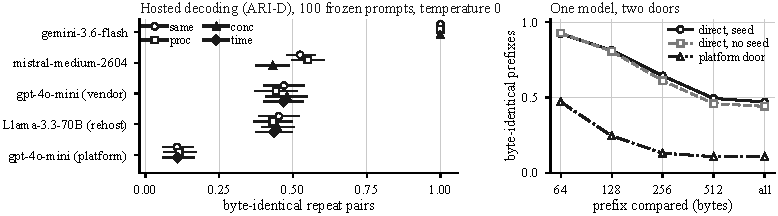
\includegraphics[width=\linewidth]{figure2.pdf}
\caption{Left: repeat rates with 95\% CIs. Right: the same model snapshot via vendor API and a gateway. (Existing figure; probe-independent.)}\label{fig:arid}
\end{figure}
\begin{itemize}
  \item Repeatability at temperature 0 is far from 1.0 for 4 of 5 endpoints; one vendor holds 1.000 over 2{,}800 completions incl.\ a 64-way burst.
  \item Same snapshot, two doors: gateway half as byte-stable at 64 bytes, 4$\times$ less over full completions; no-seed control does not close the gap.
  \item No condition separates from \texttt{same} under the CI rule; power: a 0.10 drop is detected at 0.89--0.97 if bimodal, 0.53--0.55 if concentrated.
  \item Orderings differ between layers (Mistral below OpenAI on embeddings, above on generation) $\Rightarrow$ measure each layer.
\end{itemize}

%=====================================================================
\section{Using ARI}\label{sec:use}
\begin{table}[h]\centering\footnotesize
\caption{Practitioner guide.}\label{tab:guide}
\begin{tabular}{p{0.34\linewidth}p{0.18\linewidth}p{0.38\linewidth}}
\toprule
question & run & read \\
\midrule
Will my stored embeddings/IDs still match after a restart? & \texttt{proc} & HER$_{\texttt{proc}}$; $<1$ means re-encode or tolerate mismatches \\
Does traffic load change outputs? & \texttt{conc} & HER$_{\texttt{conc}}$ vs HER$_{\texttt{same}}$ \\
Will results match next week? & \texttt{time} & HER$_{\texttt{time}}$; repeat periodically \\
Which provider/model drifts less? & core three & ARI-R ($1-\bar\rho$), never HER \\
Is my self-hosted stack deterministic? & \texttt{proc}, \texttt{mach} & expect 1.000 at fp32, TF32 off \\
Did a precision/serving change happen? & \texttt{prec} & $\rho$ jumps by orders of magnitude \\
Is my LLM API stable at temp 0? & ARI-D & exact-repeat rate per condition \\
\bottomrule
\end{tabular}
\end{table}
\begin{itemize}
  \item \texttt{pip install ari-benchmark} (pulls \texttt{semq==1.0.0}); one command per condition; report validates against the public schema; verify with the standalone verifier. \todo{exact commands}
  \item Interpretation rules: HER = 1.000 means exact codes, not semantic equality or quality; compare only reports with matching inputs, probe version and conditions.
\end{itemize}

%=====================================================================
\section{Limitations}
\begin{itemize}
  \item One realization per condition on APIs; CIs cover inputs, not serving states. \todo{weekly repeats}
  \item $\rho$ normalization verified 384--1{,}024-d; isotropic noise model.
  \item The code is a threshold detector by design: sub-threshold changes are invisible (Fig.~\ref{fig:selectivity}); use a hash if any bit matters.
  \item ARI-D is a dry run: two endpoints lack \texttt{time}.
  \item Operator-signed reports prove integrity and origin, not neutrality.
\end{itemize}

\section{Conclusion}
\begin{itemize}
  \item Two layers, one protocol, two numbers (HER for ``does it match'', $\rho$ for ``how much does it move'').
  \item \todo{one-paragraph conclusion after reruns}
\end{itemize}

\section*{References}
\small
[1] He, H. and Thinking Machines Lab. Defeating Nondeterminism in LLM Inference. 2025.
[2] Yuan, J. et al. Understanding and Mitigating Numerical Sources of Nondeterminism in LLM Inference. arXiv:2506.09501, 2025.
[3] Rajput, S. et al. Recommender Systems with Generative Retrieval. NeurIPS 2023.
[8] Yashwanth, T. S. On the Structure of Floating-Point Noise in Batch-Invariant GPU Matrix Multiplication. arXiv:2511.00025, 2025.
\todo{carry over remaining references}
\normalsize

\appendix
%=====================================================================
\section{Probe design evidence}\label{app:probe}
\begin{table}[h]\centering\footnotesize
\caption{Calibrated (v0.1) vs fixed-range (v0.2) probe, 8 encoders, $n_{\text{bins}}=2$.}
\begin{tabular}{lcc}
\toprule
measure & calibrated & fixed-range \\
\midrule
false positives & 0 & 0 \\
bf16 changes detected (10 cells) & 88.2--99.9\% & 93.1--100\% \\
Spearman(L2 drift, coordinates changed) & 0.864--0.946 & 0.875--0.947 \\
codes changed by recalibrating on another corpus slice & 60--100\% & 0\% (no calibration) \\
needs a per-model scale & yes & no \\
\bottomrule
\end{tabular}
\end{table}
\begin{figure}[h]\centering
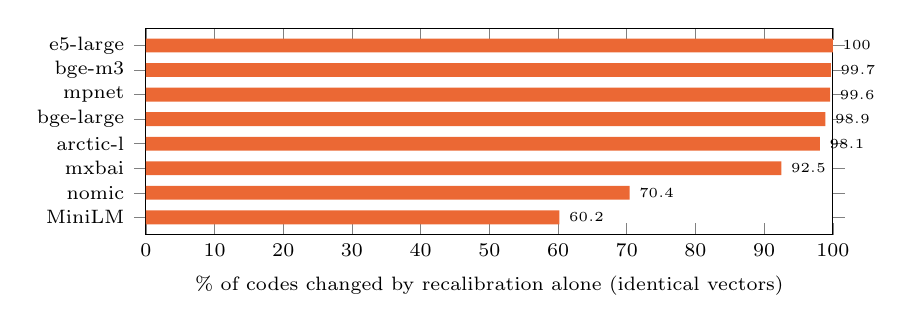
\begin{tikzpicture}
\begin{axis}[xbar, bar width=5pt, width=0.85\linewidth, height=4.2cm, xmin=0, xmax=100, xlabel={\% of codes changed by recalibration alone (identical vectors)},
  symbolic y coords={MiniLM,nomic,mxbai,arctic-l,bge-large,mpnet,bge-m3,e5-large}, ytick=data,
  tick label style={font=\scriptsize}, label style={font=\scriptsize}, nodes near coords, nodes near coords style={font=\tiny}]
\addplot[fill=sTwo, draw=none] coordinates {(60.2,MiniLM)(70.4,nomic)(92.5,mxbai)(98.1,arctic-l)(98.9,bge-large)(99.6,mpnet)(99.7,bge-m3)(100,e5-large)};
\end{axis}
\end{tikzpicture}
\caption{Calibrated probe: scale from FiQA rows vs SciFact rows of the same input set. The fixed-range probe has no such dependence.}
\end{figure}

\section{ARI-D-internal: the logit probe}\label{app:logit}
\begin{itemize}
  \item Centre each logit row over the vocabulary; split at fixed 65{,}536-wide chunks; encode each chunk with QUANT, 8 bins.
  \item Invariant to a constant logit shift (softmax-invariant); chunk layout fixed by vocabulary size.
  \item Use when internal drift below the argmax matters; a top-2 margin is a cheaper monitor for decision changes.
\end{itemize}
\begin{table}[h]\centering\footnotesize
\caption{Probe choice on Qwen2.5-0.5B logits (151{,}936 vocab, 640 rows).}
\begin{tabular}{lrrr}
\toprule
 & calibrated & no centring & v0.2 (centred) \\
\midrule
detects GPU fp32 change & 71.3\% & 76.4\% & \textbf{82.5\%} \\
codes changed by +3 on every logit & 100\% & 100\% & \textbf{1.7\%} \\
Spearman with centred drift (bf16/int8) & 0.53--0.74 & 0.45--0.51 & \textbf{0.84--0.86} \\
Spearman with raw drift (bf16/int8) & \textbf{0.96} & 0.57--0.67 & 0.54--0.70 \\
\bottomrule
\end{tabular}
\end{table}
\begin{table}[h]\centering\footnotesize
\caption{Decoding, 48 prompts $\times$ 48 tokens, greedy, one L40S, v0.2. bf16: $<$1\% of tokens change, 21--42\% of generations differ.}
\begin{tabular}{llrrr}
\toprule
model & condition & token agreement & logit HER & generations identical \\
\midrule
Llama-3.1-8B & proc / threads / TF32 off & 100\% & 1.000 & 48/48 \\
 & TF32 on & 100\% & 0.000 & 48/48 \\
 & batched (pad to 4) & 100\% & 0.400 & 48/48 \\
 & fp16 & 99.96\% & 0.000 & 46/48 \\
 & bf16 & 98.90\% & 0.000 & 33/48 \\
Qwen2.5-7B & proc / threads / TF32 off & 100\% & 1.000 & 48/48 \\
 & TF32 on & 99.96\% & 0.000 & 48/48 \\
 & batched (pad to 4) & 100\% & 0.251 & 48/48 \\
 & fp16 & 99.87\% & 0.000 & 43/48 \\
 & bf16 & 99.03\% & 0.000 & 28/48 \\
Mistral-7B-v0.3 & proc / threads / TF32 off & 100\% & 1.000 & 48/48 \\
 & TF32 on & 100\% & 0.000 & 48/48 \\
 & batched (pad to 4) & 100\% & 0.674 & 48/48 \\
 & fp16 & 99.96\% & 0.000 & 44/48 \\
 & bf16 & 99.38\% & 0.000 & 38/48 \\
\bottomrule
\end{tabular}
\end{table}

\section{Probe vs alternatives at matched storage}\label{app:matched}
\begin{itemize}
  \item Planned: code vs SHA-256, block hashes, cosine, top-$k$, KL/JS, top-2 margin, fp16 reference at equal bytes; 300 control + 300 intervention episodes; alarm rate fixed on controls.
  \item Pilot (12 prompts) is degenerate: two interventions were bit-identical, two were caught by everything, controls produced no alarms.
  \item \todo{define ``material'' vs ``benign'' change before the confirmatory run (see Fig.~\ref{fig:selectivity})}
\end{itemize}

\section{Corrections to the v0.1 pipeline}
\begin{itemize}
  \item Model dtype not enforced (mxbai ran in fp16); now loaded in an explicit, verified dtype.
  \item One capture measured bf16 by in-place cast; now a fresh bf16 load.
  \item Self-hosted \texttt{time} was a same-session repeat; now a stored baseline compared $\ge$24\,h later.
  \item A measured \texttt{conc} flip was recorded as 1.000; values are now recorded as measured.
\end{itemize}

\section{Reproducibility}
\begin{itemize}
  \item Harness Apache-2.0; spec and inputs CC BY 4.0; SEMQ SDK public (PolyForm Noncommercial 1.0.0, \texttt{semq==1.0.0}).
  \item Reports signed by the registered KMS key; standalone verifier imports neither the harness nor the SDK.
  \item \todo{commit hashes and S3/DOI for raw vectors}
\end{itemize}

\end{document}
